\documentclass[12pt,a4paper]{article}

% Margins.
\setlength{\oddsidemargin}{0in}
\setlength{\evensidemargin}{0in}
\setlength{\headheight}{12pt}
\setlength{\headsep}{42pt}
\setlength{\topmargin}{-54pt}
\setlength{\textwidth}{6.5in}
\setlength{\textheight}{10in}
\pagestyle{plain}

\usepackage{amsmath}
\usepackage{float}
\usepackage{graphicx}
\usepackage[hyphens]{url}
\usepackage[hidelinks]{hyperref}	% Clickable links to figures, references and urls.
\usepackage{lastpage}

% Drawing.
\usepackage{pgf}
\usepackage{tikz}

% Listings for formatting code.
\usepackage{listings}
\usepackage{textcomp}
% General options.
\lstset{breaklines=true, basicstyle=\small\ttfamily, tabsize=4, numbers=left, stepnumber=1, frame=single, showstringspaces=false, upquote=true}
% C++ specific high-lighting. Comments are 50/50 shades of green/black and strings coloured with 60/40 red/black mixture.
\lstset{language=[ISO]C++, commentstyle=\color{green!50!black}, keywordstyle=\color{blue}, stringstyle=\color{red!60!black}}

% Marks of each question.
\def\QOne{5}
\def\Qtwo{10}
\def\Qthree{20}
\def\Qfour{15}
\def\Qfive{30}
\def\Qsix{20}
\def\TotalMarks{100}

\begin{document}
\begin{minipage}{0.55\textwidth}
{\LARGE \textbf{Programming for\\ Engineers II}}\\[0.15cm]
{\normalsize \textbf{Summer 2013 Semester}}\\
{\Large {Sessional Exam}}\\
{\normalsize \textbf{Saturday, July 07, 2013}}\\[0.30cm]
{\Large \textbf{Total Time: 90 minutes}}\\[0.15cm]
{\Large \textbf{Total Marks: 100}}\\
\textbf{Course Instructor:}\\
Attique Dawood\\
\end{minipage}
\begin{minipage}{0.4\textwidth}
\textbf{Serial} \hrulefill \\[0.25cm]
\textbf{Name} \hrulefill\\[0.25cm]
\textbf{Section} \rule{1cm}{0.2mm} \textbf{Roll No:} \hrulefill\\[0.25cm]
\textbf{Signature:} \hrulefill\\[0.25cm]
\rule{6.6cm}{0.2mm}\\
\textbf{Signature of Invigilator}\\[0.25cm]
\end{minipage}
\begin{table}[H]
\begin{center}
\vspace{0.3cm}
	{\Large \begin{tabular}{|c|c|c|c|c|c|c|c|}
	\hline
		\rule{0pt}{2.6ex} Question & \textbf{1} & \textbf{2} & \textbf{3} & \textbf{4} & \textbf{5} & \textbf{6} & \textbf{Total}\\
		\hline
		Total Marks \rule{0pt}{2.6ex} & \QOne & \Qtwo & \Qthree & \Qfour & \Qfive & \Qsix & \TotalMarks\\
		\hline
		Marks Obtained & & & & & & &\\
	\hline
	\end{tabular}}
\end{center}
\end{table}
\noindent \textbf{You are advised to READ these notes:}
\begin{enumerate}
\item \textbf{Attempt on the Question Paper. \underline{NO EXTRA SHEET} will be provided/accepted. No
additional sheet will be provided for rough work. Use the back of the page where
provided space is not sufficient.}
\item After asked to commence the exam, please verify that you have \textbf{\pageref{LastPage} different
printed pages} including this title page.
\item There are 6 questions. Attempt all of them. It is advisable to go through the paper once
before starting with the first question.
\item Exam is closed books, closed notes. Please see that the area in your threshold is clean.
You will be charged for any material which can be classified as \textbf{`helping in the paper'}
found near you.
\item \textbf{Calculator sharing is strictly prohibited.}
\item Students who attempt the paper with lead pencils lose the right to get them rechecked.
\item \textbf{The invigilator present is not supposed to answer any questions. No one may come
to your room for corrections and you are not supposed to request to call anyone.
Make assumptions wherever required and clearly mark them.}
\end{enumerate}
\newpage
\noindent\textbf{Question 1: Simple Output\hfill \QOne~marks}\\
Write the output of following code snippet.
\begin{lstlisting}
#include <iostream>
using namespace std;

int main()
{
	int x = 3;
	char c = '3';
	cout << "x is " << x << " and c is " << c << endl;
	
	return 0;
}
\end{lstlisting}
\begin{figure}[H]
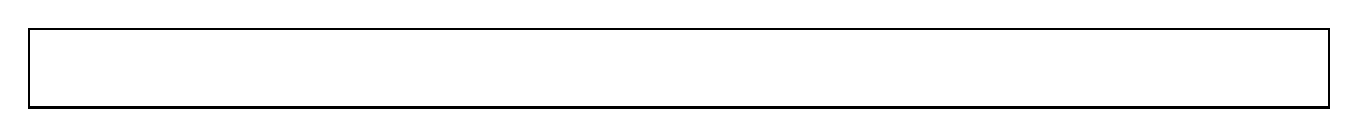
\begin{tikzpicture}
	\draw[thick] (0cm,0cm) rectangle (\textwidth, 1cm);
\end{tikzpicture}
\end{figure}

\noindent\textbf{Question 2: Compilation Steps \hfill \Qtwo~marks}\\
What are the different steps involved in programming cycle (from editing to creation of executable)? 
\begin{figure}[H]
\begin{tikzpicture}
	\draw[thick] (0cm,0cm) rectangle (\textwidth, 3cm);
\end{tikzpicture}
\end{figure}

\noindent\textbf{Question 3: Bitwise and Shift Operators \hfill $4\times 5=$\Qthree~marks}\\
Assume 4 bit unsigned binary numbers. Evaluate the following:
\begin{enumerate}
\item \verb|4 & 5|
\item \verb$4 | 7$
\item \verb|3 ^ 9|
\item \verb|7 >> 2|
\item \verb|8 << 1|
\end{enumerate}
\begin{figure}[H]
\begin{tikzpicture}
	\draw[thick] (0cm,0cm) rectangle (\textwidth, 5cm);
\end{tikzpicture}
\end{figure}

\noindent\textbf{Question 4: Signed Integers \hfill \Qfour~marks}\\
Assuming 16 bit signed integer, what is the bit representation of -147? Show how this number is stored in computer memory.
\begin{figure}[H]
\begin{tikzpicture}
	\draw[thick] (0cm,0cm) rectangle (\textwidth, 10cm);
\end{tikzpicture}
\end{figure}

\noindent\textbf{Question 5: Float Representation \hfill $15+15=$\Qfive~marks}\\
a. Convert 37.390625 to 32 bit floating point representation. Also show how this number is stored in computer memory.
\begin{figure}[H]
\begin{tikzpicture}
	\draw[thick] (0cm,0cm) rectangle (\textwidth, 10cm);
\end{tikzpicture}
\end{figure}
\noindent b. Convert the following 32 bit floating point number into decimal.\\
\verb|1 10000110 10110110000000000000000|
\begin{figure}[H]
\begin{tikzpicture}
	\draw[thick] (0cm,0cm) rectangle (\textwidth, 8cm);
\end{tikzpicture}
\end{figure}
\noindent\textbf{Question 6: Loops \hfill \Qsix~marks}\\
Write C++ code to input an integer from user and determine if it is a prime number.
\begin{figure}[H]
\begin{tikzpicture}
	\draw[thick] (0cm,0cm) rectangle (\textwidth, 12cm);
\end{tikzpicture}
\end{figure}
\end{document}